\documentclass[10pt]{beamer}

\usetheme[progressbar=frametitle]{metropolis}
\usepackage[italian]{babel}

\usepackage{appendixnumberbeamer}

\usepackage{booktabs}
\usepackage[scale=2]{ccicons}

\usepackage{pgfplots}
\usepgfplotslibrary{dateplot}

\usepackage{xspace}
\newcommand{\themename}{\textbf{\textsc{metropolis}}\xspace}

\title{Soccer Activities Management}
\subtitle{Progetto del corso di Ingegneria del Software Avanzata}
\date{13 settembre 2022}
\author{Michele Vaccari - Matricola 121955}
\institute{Università degli studi di Ferrara\\Corso di laurea magistrale in Ingegneria Informatica e dell'Automazione\\AA 2021-2022}

% logo of my university
\titlegraphic{%
  \begin{picture}(0,0)
    \put(305,0){\makebox(0,0)[rt]{
\includegraphics[width=4cm]{../images/logo-unife}}}
  \end{picture}}

\begin{document}

\maketitle

\begin{frame}{Indice}
  \setbeamertemplate{section in toc}[sections numbered]
  \tableofcontents[hideallsubsections]
\end{frame}

\section{Processo di ingegneria dei requisiti}

\begin{frame}{Descrizione}
Il sito \emph{Soccer Activities Management} è una piattaforma per la gestione delle attività sportive attraverso una comunità di utenti.
\end{frame}

\begin{frame}[allowframebreaks]{Caratteristiche}
\begin{enumerate}
	
	\item
	\label{sf-uadmin}
	Possibilità di creare gli utenti per i due ruoli principali: arbitri e gestori di squadra
	
	\item
	Possibilità di creare i diversi tornei, di disegnarne lo schema. Ogni torneo ha: nome, descrizione e tipo (all'italiana o ad eliminazione)
	
	\item
	Un torneo è costituito da diversi gironi o fasi, in base alla tipologia di torneo. Un girone ha un nome (ad esempio: girone 1) ed è costituito da un insieme di gare. Una fase ha un nome (ad esempio: semifinale 1) ed è costituita da una sola gara
	
	\item
	Una gara è descritta da: data e ora, luogo, nomi delle squadre che si sfidano, un arbitro
	
	\item
	\label{ef-uadmin}
	Per ogni torneo è associata una classifica generale che viene aggiornata sulla base dei referti di gara compilati dagli arbitri

	\item
	\label{sf-ugestore}
	Possibilità per il gestore di una squadra di creare una squadra con una rosa di massimo 36 giocatori. Ogni squadra ha un nome e può avere uno sponsor. Per ogni giocatore il gestore può specificare: nome, cognome, luogo e data di nascita, numero di maglia e foto
	
	\item
	\label{ef-ugestore}
	Per ogni gara cui la squadra è assegnata, il gestore della squadra deve fornire la formazione della squadra composta da nome e cognome dei giocatori e rispettivi ruoli
	
	\item
	\label{f-uarbitro}
	A gara terminata l'arbitro dovrà compilare un referto in cui annoterà: l'orario effettivo di inizio e di fine della gara, risultato finale, numero di reti con i rispettivi giocatori che li hanno realizzati,  i giocatori espulsi per ogni squadra e i giocatori ammoniti per ogni squadra
	
\framebreak

	\item
	\label{f-upubblico}
	Possibilità di selezionare il torneo desiderato e visualizzare:
	
	\begin{itemize}
		\item 
		La pagina relativa ad una gara con: nomi delle squadre, formazioni e referti
		
		\item
		La pagina relativa ad una squadra con la rosa dei giocatori e il calendario delle partite
		
		\item
		La pagina relativa ad un giocatore con le statistiche di gioco (punti realizzati, espulsioni e ammonizioni) per quel torneo
	\end{itemize}

\end{enumerate}
\end{frame}

\begin{frame}{Utenti del sistema}

Il sistema prevede che le categorie di utenti sia così rappresentata:

\begin{description}
	
	\item[Amministratori] Possono effettuare i punti dal \ref{sf-uadmin} al \ref{ef-uadmin} compresi
	
	\item[Gestori di squadra] Possono effettuare i punti dal \ref{sf-ugestore} al \ref{ef-ugestore} compresi
	
	\item[Arbitri] Possono effettuare solamente il punto \ref{f-uarbitro}
	
	\item[Utenti pubblici] Possono effettuare solamente il punto \ref{f-upubblico}
	
\end{description}
\end{frame}

\section{Demo}

\begin{frame}{Demo del sistema}

Rileggiamo le specifiche e vediamo l’implementazione del sistema sviluppato utilizzando i dati demo.

\begin{table}
	\caption{Credenziali e ruoli degli utenti demo del sistema}
    \begin{tabular}{c c c c}
      \toprule
      Email & Password& Tipo & Squadra\\
      \midrule
	m.vaccari@sam.com & Password01 & Admin \\
	u.cairo@sam.com & Password01 & Team Manager & Torino \\
	w.mattioli@sam.com & Password01 & Team Manager & S.P.A.L. 2013 \\
	m.setti@sam.com & Password01 & Team Manager & Hellas Verona \\
	j.saputo@sam.com & Password01 & Team Manager & Bologna \\
	m.busacca@sam.com & Password01 & Referee \\
	p.collina@sam.com & Password01  & Referee \\
      \bottomrule
    \end{tabular}
  \end{table}

\end{frame}


\section{Licenza}

\begin{frame}{Licenza MIT}

Si è scelto di distribuire il software sviluppato tramite licenza \emph{MIT}.\\
La licenza \href{https://mit-license.org/}{MIT} è una licenza permissiva, molto semplice e breve, che permette di fare ciò che si vuole col codice a patto che la licenza venga re-distribuita nel codice che si utilizza.

\end{frame}

\section{Componenti del sistema}

\begin{frame}{Architettura software}
	\begin{figure}[h]
		\centering
		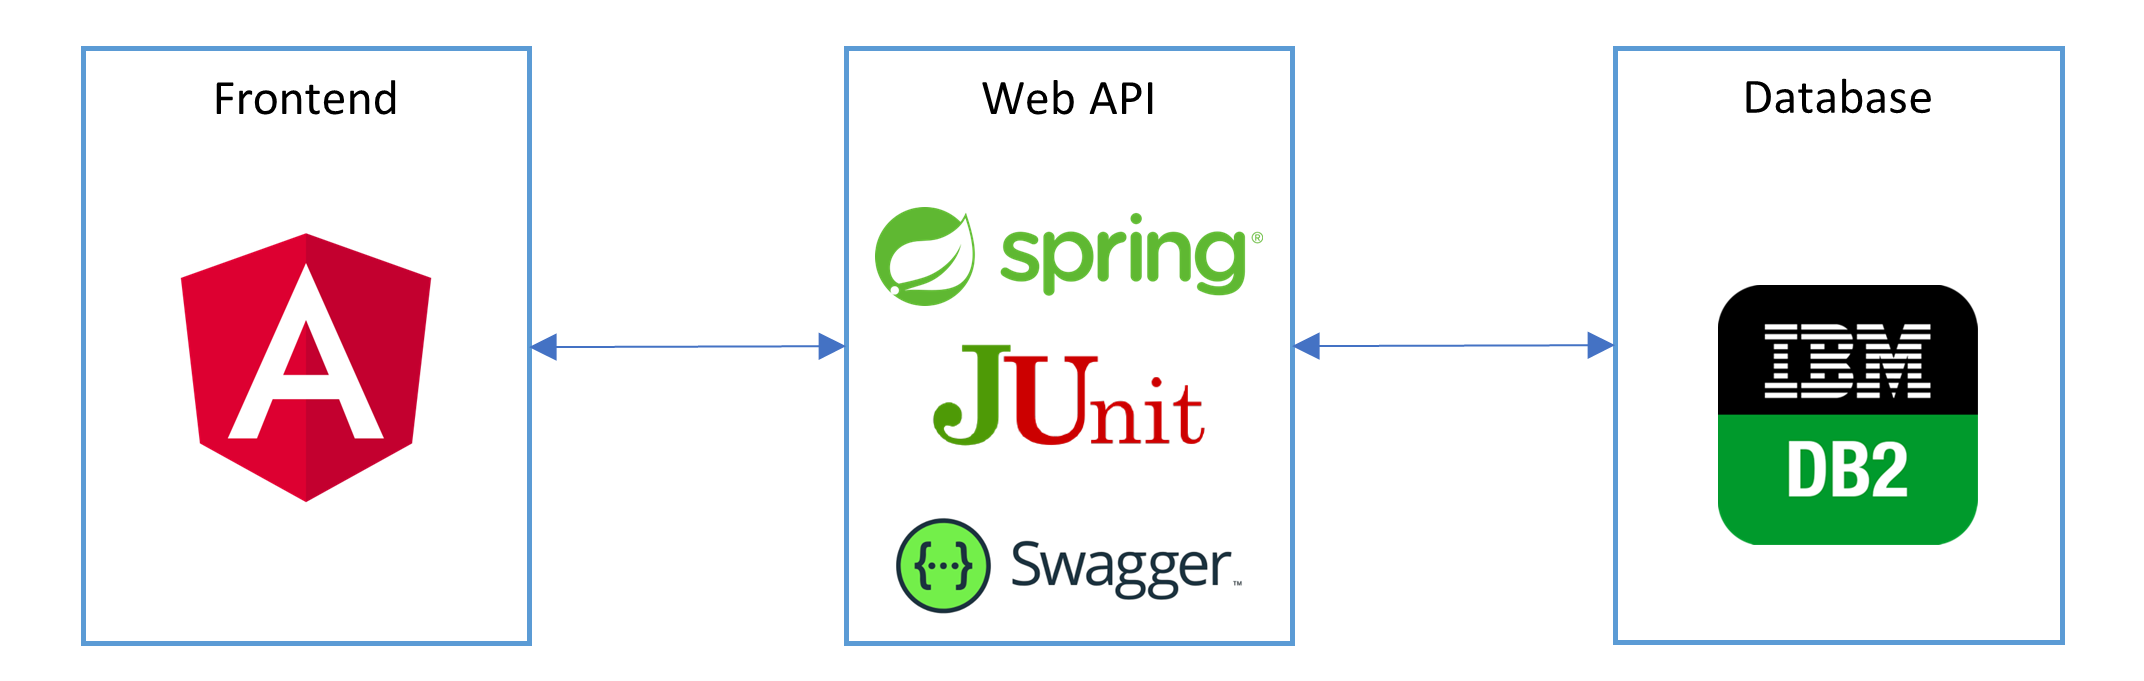
\includegraphics[width=1\textwidth]
		{../images/software-architecture-diagram}
		
		\caption{Architettura del sistema}
	\end{figure}
\end{frame}

\begin{frame}{Frontend}
	
	\begin{itemize}
	
		\item
		\textbf{Linguaggio:} \href{https://www.typescriptlang.org/}{TypeScript}
		
		\item
		\textbf{Framework:} \href{https://angular.io/}{Angular}

		\item
		\textbf{Gestore delle dipendenze:} \href{https://www.npmjs.com/}{npm} (vedi \emph{frontend/package.json})
		
		\item
		\textbf{Building system:} \href{https://nodejs.org/}{Node.js}

	\end{itemize}
	
	Le fasi di \emph{Build} e \emph{Deploy} vengono gestite utilizzando docker (vedi \emph{frontend/Dockerfile})
\end{frame}

\begin{frame}[allowframebreaks]{Database}
	
	\begin{itemize}

		\item
		\textbf{Linguaggio:} \href{https://www.w3schools.com/sql}{SQL} (\href{https://www.ibm.com/db2}{IBM Db2})

	\end{itemize}
	
	Le fasi di \emph{Build} e \emph{Deploy} vengono gestite utilizzando docker (vedi \emph{database/Dockerfile})\\
	È possible utilizzare dei dati demo per vedere l’applicazione in funzione oppure fare un’installazione pulita (vedi \emph{database/initialization-scripts})

\framebreak

	\begin{figure}
		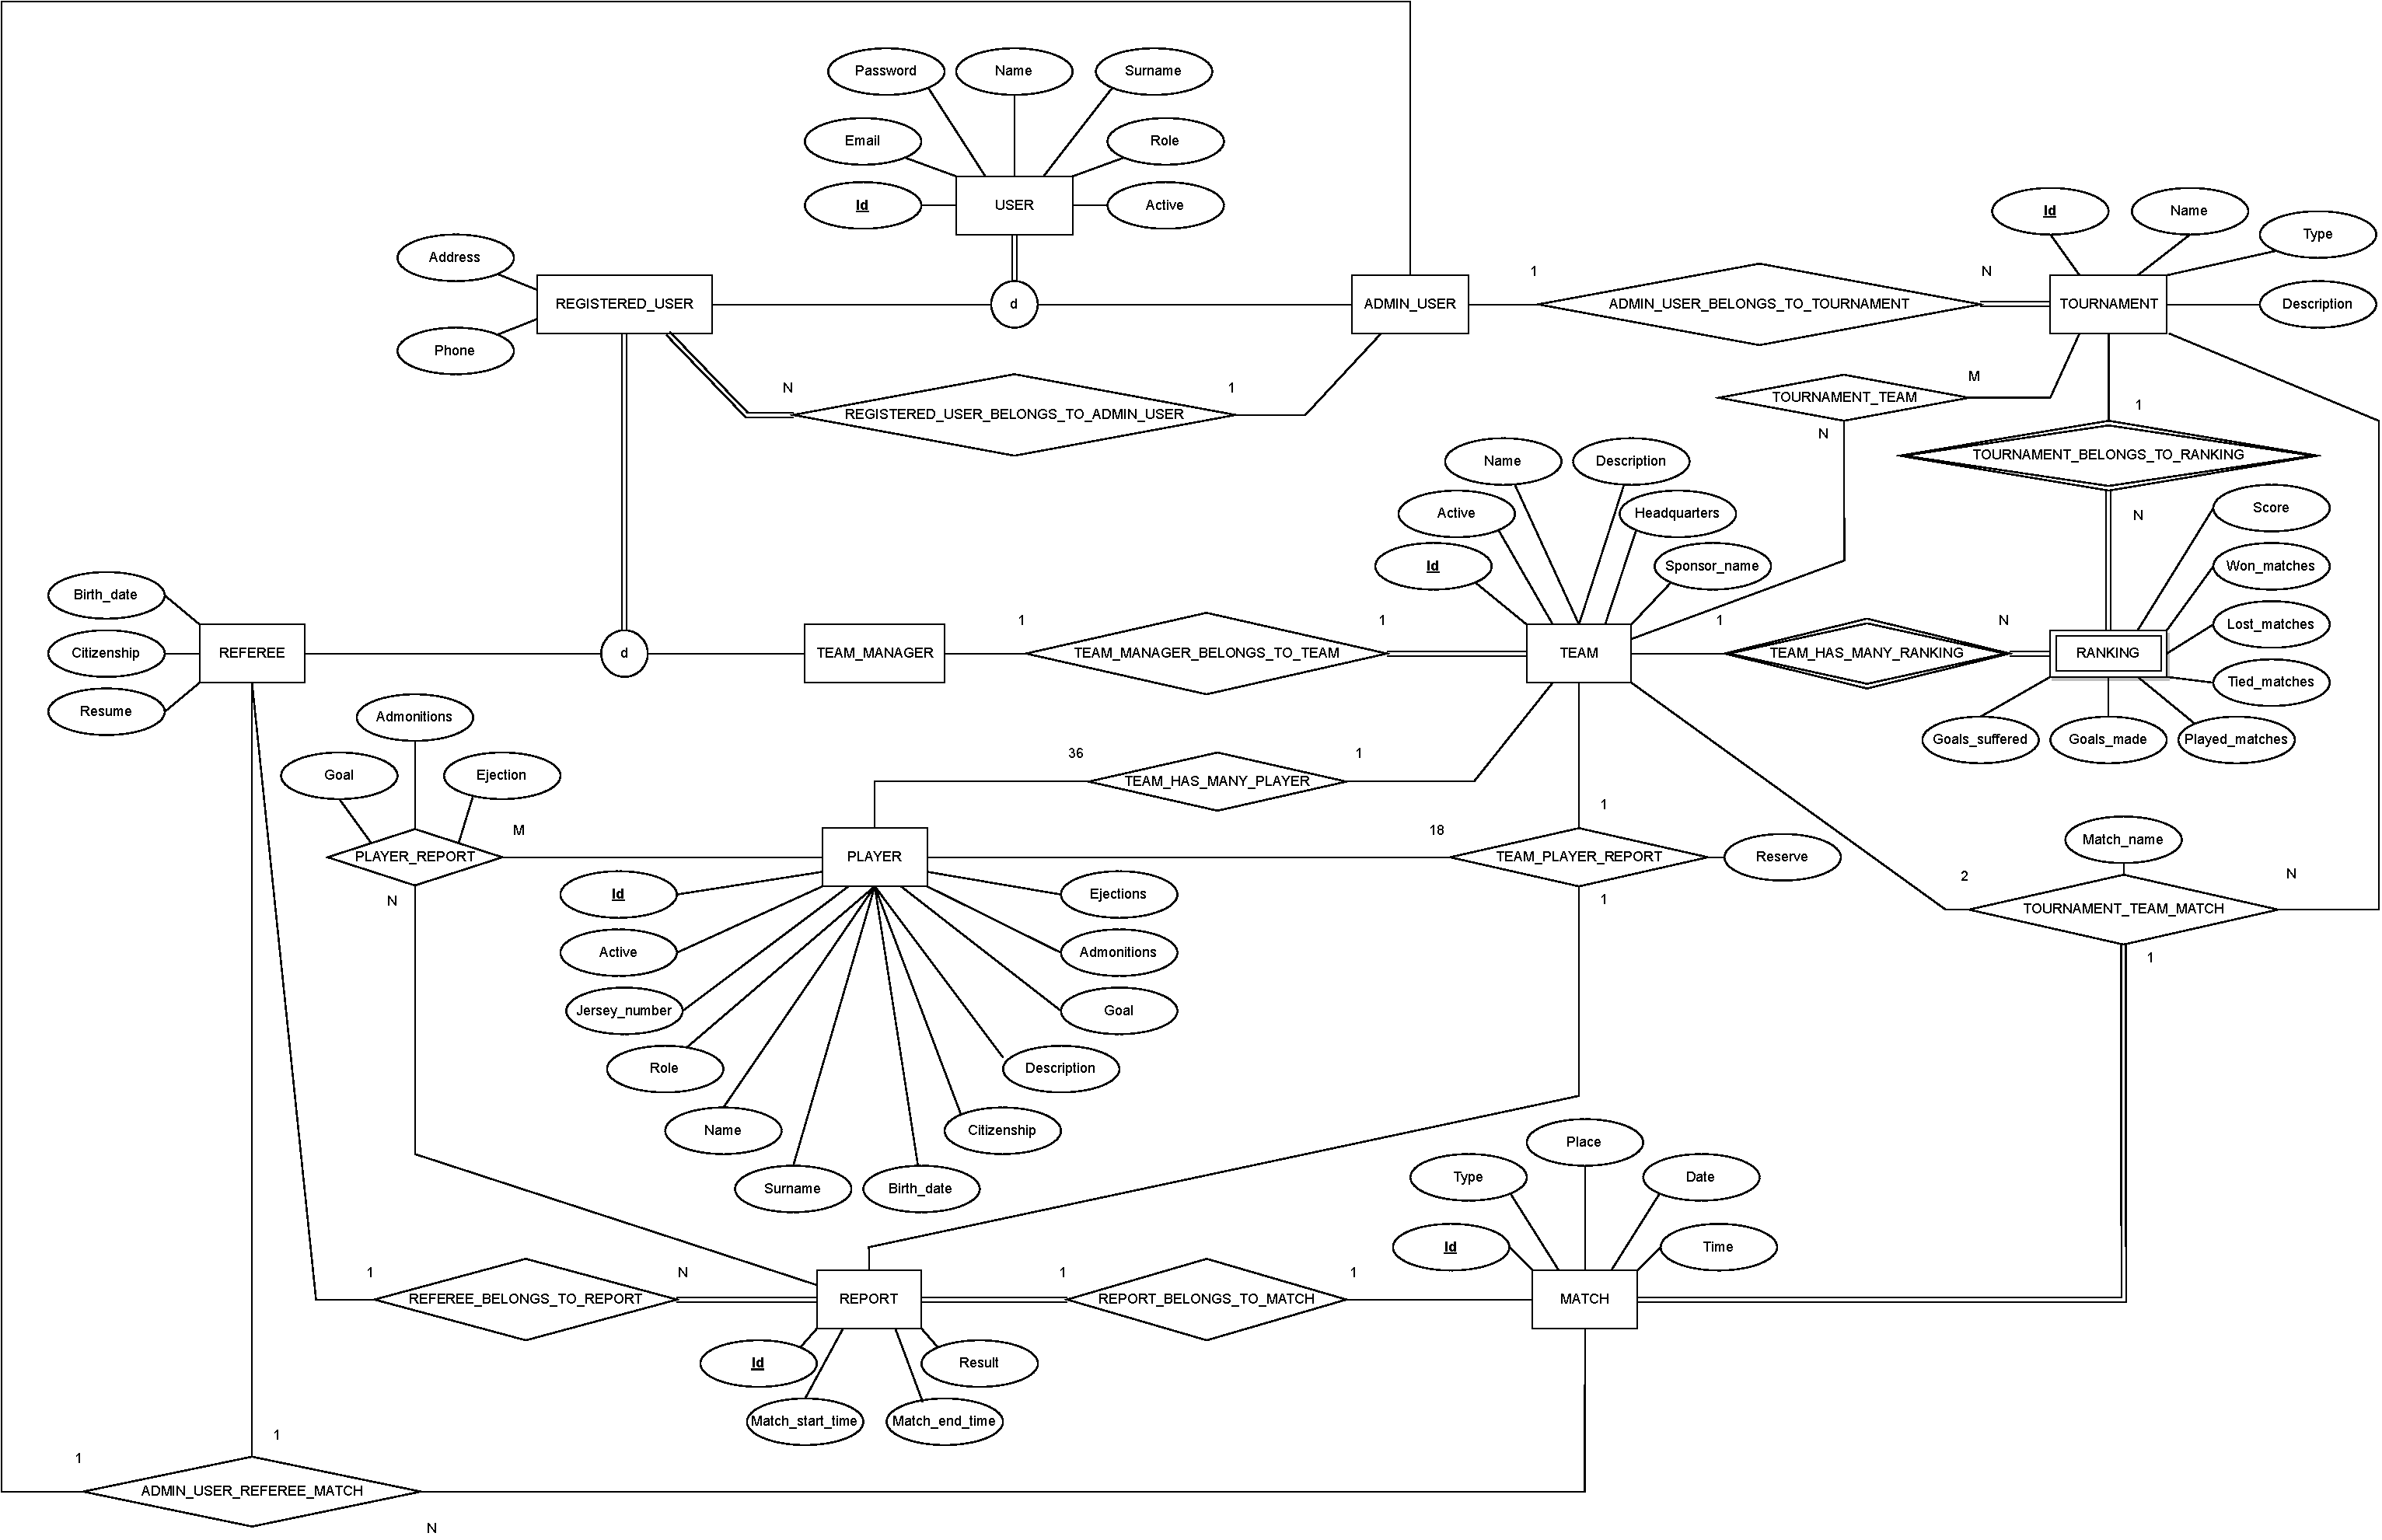
\includegraphics[width=0.8\textwidth]
		{../images/database-er-diagram}
		
		\caption{Schema ER}
	\end{figure}

\end{frame}

\begin{frame}[allowframebreaks]{Web API}

	\begin{itemize}
	
		\item
		\textbf{Linguaggio:} \href{https://docs.oracle.com/javase/7/docs/technotes/guides/language/}{Java}
		
		\item
		\textbf{Framework:} \href{https://spring.io/projects/spring-boot/}{Spring Boot}

		\item
		\textbf{Gestore delle dipendenze:} \href{https://maven.apache.org}{maven} (vedi \emph{web-api/pom.xml})
		
		\item
		\textbf{Target system:} \href{https://openjdk.org/}{OpenJDK 11}

	\end{itemize}
	
	Le fasi di \emph{Build} e \emph{Deploy} vengono gestite utilizzando docker (vedi \emph{web-api/Dockerfile})

\framebreak

	Una volta avviato il container \emph{Web API} è disponibile la documentazione delle \href{http://localhost:8080/swagger-ui.html}{API REST}

	\begin{figure}
		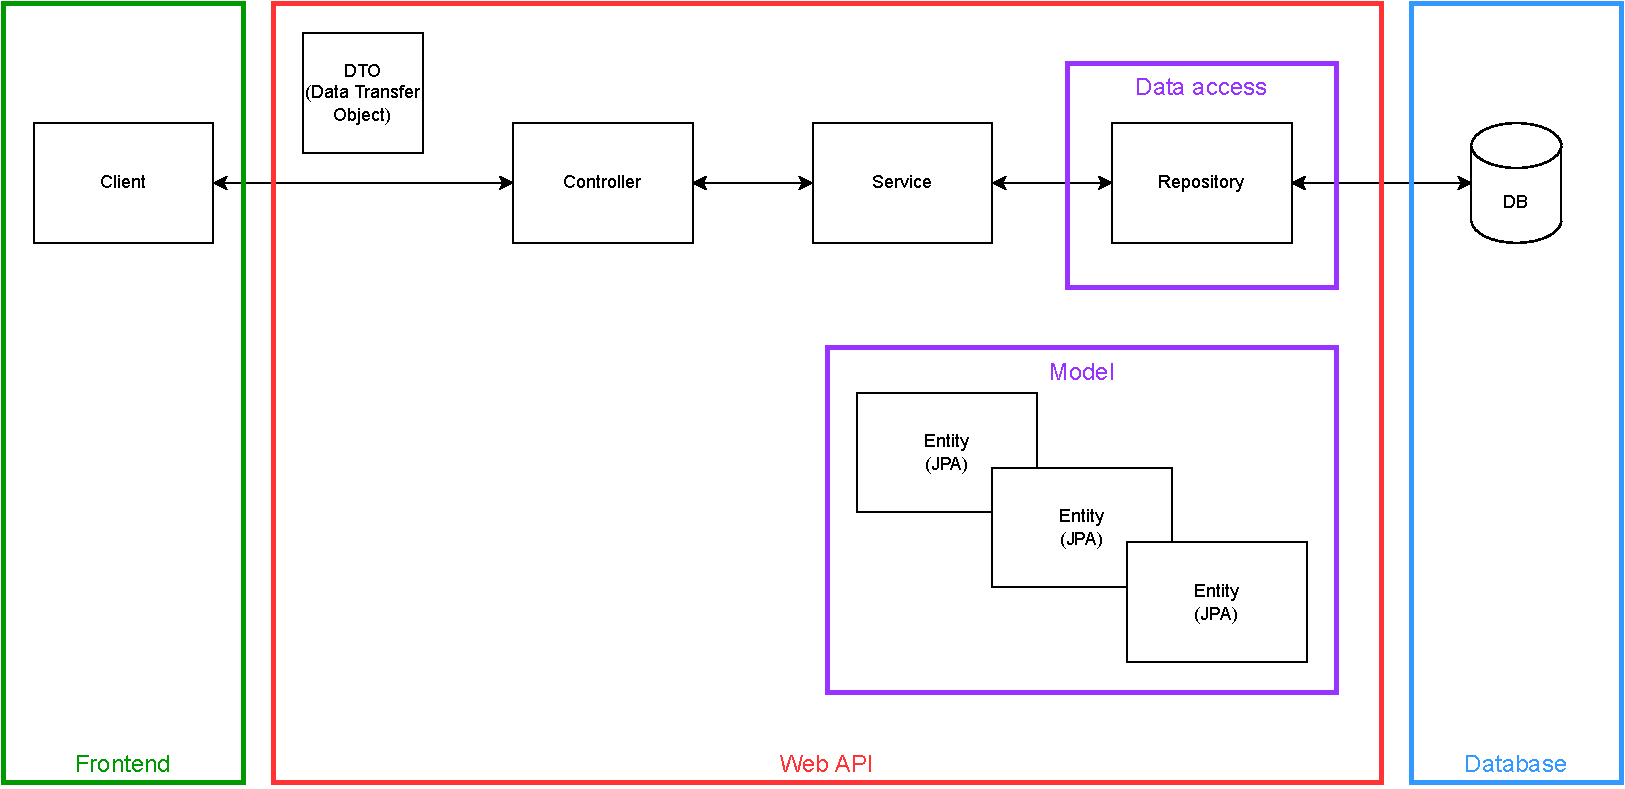
\includegraphics[width=0.8\textwidth]
		{../images/web-api-data-flow}
		
		\caption{Web API data flow}
	\end{figure}

\framebreak

	\textbf{Test White Box}\\
	\emph{Unit test (approccio bottom up):}
	\begin{itemize}

		\item
		Dto (esempio AdminDtoTest.java / AdminDto.java)
		
		\item
		Model (esempio AdminUserTest.java / AdminUser.java)

		\item
		Service (esempio AdminServiceImplTest.java / AdminServiceImpl.java)

		\item
		Controller (esempio AdminControllerTest.java / AdminController.java)

	\end{itemize}

	\emph{Difetti:}
	\begin{itemize}
	
		\item
		Copertura legata all’implementazione: una modifica dell’implementazione richiede di rivalutare i casi di test.
		
		\item
		Non rilevano la mancata implementazione di funzionalità

	\end{itemize}

	\textbf{Test Black Box} (basati sulla specifica di un modulo, anziché sulla sua implementazione)
	\begin{itemize}
		
		\item
		Come specifica del modulo utilizzare la documentazione delle \href{http://localhost:8080/swagger-ui.html}{API REST}

		\item
		Utilizzo del software \href{https://www.postman.com/}{Postmann} per creare una suite di test

	\end{itemize}

\end{frame}

\section{Tipi di processo e strumenti usati }

\begin{frame}[allowframebreaks]{Tipi di processi usatii}

Si sono utilizzati prevalentemente processi agili, in particolare si è cercato di:
\begin{itemize}
	
		\item
		Sviluppare e consegnare per incrementi: testare e valutare ogni incremento
		
		\item
		Mantenere la semplicità: limitare la complessità del sistema sia in fase di sviluppo che in fase di progettazione

		\item
		Limitare l’uso di duplicazioni di logica e l'uso di commenti \cite{martin2018clean}
\end{itemize}

Durante lo sviluppo si è seguito un tipo di processo pianificato-agilmente (uso del metodo dei \emph{proiettili traccianti}\cite{hunt2018pragmatic}): si traccia una linea guida delle attività da seguire pianificandole in anticipo. Durante l’analisi e lo sviluppo si possono sperimentare e modificare le tecnologie a disposizione (plugin e librerie) ma non i requisiti.

\framebreak

	\textbf{Extreme Programming}
	
	\begin{itemize}
		\item
		\emph{Incremental planning e user story:} non esiste un grande piano per il sistema e i requisiti vanno discussi incrementalmente con un rappresentante del cliente. I requisiti prendono anche il nome di \emph{user story} e sono determinati dal tempo disponibile e dalle diverse priorità. Dalle story nascono le funzionalità da implementare

		\item
		\emph{Small release (o meglio small feature sul branch develop):} rilasci frequenti. Si sviluppa prima un insieme minimo di funzionalità, per avere un business, poi si integrano con release successive

		\item
		\emph{Continuous integration:} integrazione continua. Appena il codice è pronto, questo viene integrato nel sistema e quindi nasce una nuova versione. Tutti i test di unità devono essere eseguiti in maniera automatica e devono avere successo affinché una nuova versione del software sia accettata

		\item
		\emph{Refactoring:} miglioramento della struttura e dell’efficienza del codice per agevolarne la manutenzione
	\end{itemize}
\framebreak

	\textbf{Integrazione e configurazione} \\
		\emph{Svantaggi (vedi caso dell’uso di Spring Security e validazione del \href{https://jwt.io/}{JWT}):}
	\begin{itemize}
		
		\item
		Non sempre il software riusabile è sufficientemente flessibile per adattarsi completamente ai requisiti con la sola configurazione (e valutare ciò a priori è difficile)
		
		\item
		Molti framework rendono banale implementare gran parte dei requisiti, ma difficile implementare i rimanenti; il risultato è che spesso si decide di lasciare non implementati i requisiti problematici

		\item
		Non si ha controllo sull’evoluzione del software riutilizzato

		\item
		È necessario adattarsi alla filosofia progettuale del software riusato

	\end{itemize}

\end{frame}

\begin{frame}{Modello di Gitflow usato}

	\begin{figure}[h]
		\centering
		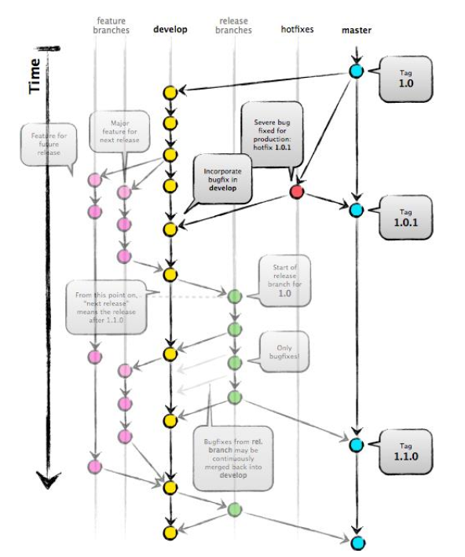
\includegraphics[width=0.5\textwidth]
		{../images/git-flow}
		
		\caption{Git flow}
	\end{figure}

\end{frame}

\begin{frame}{Convalida e Verifica dei componenti}

	\textbf{Frontend}
	\begin{itemize}

		\item
		Code walkthroughs (esecuzioni manuali)

		\item
		Code reviews (prima di mergiare una PR) 

	\end{itemize}

	\textbf{Web API}
	\begin{itemize}

		\item
		Approccio White Box

		\item
		Apporccio Black Box

		\item
		Code walkthroughs (esecuzioni manuali)

		\item
		Code reviews (ispezioni alla ricerca di errori o regole di codifica non rispettate)

	\end{itemize}

	\textbf{Database}
	\begin{itemize}

		\item
		Code walkthroughs (esecuzioni manuali)

		\item
		Code reviews (prima di mergiare una PR)

	\end{itemize}

\end{frame}

\begin{frame}{Continuous Integration}

	\textbf{Continuous integration (CI):} non appena lo sviluppatore completa un task, le modifiche vengono integrate nel sistema (push nel repository remoto). Dopo l’integrazione il sistema viene compilato (build del sistema) e vengono eseguiti tutti i test in maniera automatica. Il codice può essere poi integrato nel branch principale (main, master o altro nome).


	\textbf{GitHub actions}\\
	Vedi:
	\begin{itemize}
	
		\item
		CI Frontend \emph{.github/workflows/frontend.yml}
		
		\item
		CI Web API \emph{.github/workflows/web-api.yml}

	\end{itemize}

\end{frame}

\section{Conclusioni}

\begin{frame}{Possibili sviluppi}

	\begin{itemize}

		\item
		Implementare Continuos Delivery (branch main $\rightarrow$ stable, branch release $\rightarrow$ beta, branch develop $\rightarrow$ alpha)

		\item		
		Implementare Continuos Deployment (identificare cloud provider dove deployare gli artefatti prodotti)

		\item
		Campagna di beta tester

		\item
		Potenziare la parte di test automatici

		\item
		Tool per tracciare le dipendenze in modo eterogeneo, utile anche per notifica e valutazione delle vulnerabilità di sicurezza (ad esempio \href{https://dependencytrack.org/}{Dependency Track}

		\item
		Introduzione di uno strumento per code coverage (ad esempio \href{https://www.sonarqube.org/}{SonarQube})

		\item
		Integrazione nella pipeline della generazione di documentazione software (preferibilmente redatta da un technical wiriter, utilizzando un tool come \href{https://www.sphinx-doc.org/}{Sphinx})

	\end{itemize}

\end{frame}

\begin{frame}{Considerazioni}
	\begin{itemize}
		
		\item
		Semplicità vs. Astrazione (duplicazione e logica vs generalizzazione)

		\item		
		Più un codice è generico e più test automatici chiameranno quel codice

		\item
		Test automatici vs test manuali

		\item
		Performance vs manutenibilità

	\end{itemize}
\end{frame}

\begin{frame}[allowframebreaks]{Bibliografia}

  \bibliography{bibliografia.bib}
  \bibliographystyle{abbrv}

\end{frame}

\begin{frame}[standout]
Grazie per l'attenzione
\end{frame}

\end{document}